\documentclass[12pt, titlepage]{article}

\usepackage{fullpage}
\usepackage[round]{natbib}
\usepackage{multirow}
\usepackage{booktabs}
\usepackage{tabularx}
\usepackage{longtable}
\usepackage{tikz}
\usetikzlibrary{arrows.meta, backgrounds}
\usepackage{graphicx}
\usepackage{float}
\usepackage{hyperref}
\hypersetup{
    colorlinks,
    citecolor=blue,
    filecolor=black,
    linkcolor=red,
    urlcolor=blue
}

\input{../../Comments.text}
\input{../../Common.text}

\newcounter{acnum}
\newcommand{\actheacnum}{AC\theacnum}
\newcommand{\acref}[1]{AC\ref{#1}}

% Unlikely changes are ULC, not UC, because the SRS uses UC for use cases.
\newcounter{ucnum}
\newcommand{\uctheucnum}{ULC\theucnum}
\newcommand{\uref}[1]{ULC\ref{#1}}

\newcounter{mnum}
\newcommand{\mthemnum}{M\themnum}
\newcommand{\mref}[1]{M\ref{#1}}

\begin{document}

\title{Module Guide for \progname{}} 
\author{\authname}
\date{\today}

\maketitle

\pagenumbering{roman}

\section{Revision History}

\begin{tabularx}{\textwidth}{>{\raggedright\arraybackslash}p{3cm}
>{\raggedright\arraybackslash}p{3.3cm}>{\raggedright\arraybackslash}X}
\toprule \textbf{Date} & \textbf{Developer(s)} & \textbf{Change}\\
\midrule
9 November 2026 & Moustafa Moustafa & Added the reference material, the
introduction and the anticipated and unlikely changes (\#297).\\
9 November 2026 & Moustafa Moustafa & Added the module hierarchy, the
connection between requirements and design and the module decomposition
(\#298).\\
9 November 2026 & Moustafa Moustafa & Added the traceability matrices and the
uses hierarchy diagram (\#299).\\
\bottomrule
\end{tabularx}

\newpage

\section{Reference Material}

This section records information for easy reference. 

\subsection{Abbreviations and Acronyms}

\renewcommand{\arraystretch}{1.2}
\begin{tabular}{l l} 
  \toprule		
  \textbf{symbol} & \textbf{description}\\
  \midrule 
  AC & Anticipated Change\\
  DAG & Directed Acyclic Graph \\
  FR & Functional Requirement (SRS)\\
  LC & Likely Change (SRS)\\
  M & Module \\
  MG & Module Guide \\
  MIS & Module Interface Specification\\
  NFR & Non-Functional Requirement (SRS)\\
  OS & Operating System \\
  SAF & Safety-Critical Requirement (SRS)\\
  SRS & Software Requirements Specification\\
  \progname & The drawing practice website this MG describes\\
  ULC & Unlikely Change \\
  \bottomrule
\end{tabular}\\

\newpage

\tableofcontents

\listoftables

\listoffigures

\newpage

\pagenumbering{arabic}

\section{Introduction}

Decomposing a system into modules is a commonly accepted approach to developing
software.  A module is a work assignment for a programmer or programming
team~\citep{ParnasEtAl1984}.  We advocate a decomposition
based on the principle of information hiding~\citep{Parnas1972a}.  This
principle supports design for change, because the ``secrets'' that each module
hides represent likely future changes.  Design for change matters for
\progname{} because several parts are expected to change: the lessons, the
supported devices, the refinement service and the feedback the child sees
(SRS Section~27~\citep{SRS}).

Our design follows the rules laid out by \citet{ParnasEtAl1984}, as follows:
\begin{itemize}
\item System details that are likely to change independently should be the
  secrets of separate modules.
\item Each data structure is implemented in only one module.
\item Any other program that requires information stored in a module's data
  structures must obtain it by calling access programs belonging to that module.
\end{itemize}

After completing the first stage of the design, the Software Requirements
Specification (SRS), the Module Guide (MG) is developed~\citep{ParnasEtAl1984}. The MG
specifies the modular structure of the system and is intended to allow both
designers and maintainers to easily identify the parts of the software. The
requirements the modules meet are in the SRS~\citep{SRS}, and the interface of
each module is in the MIS~\citep{MIS}. The
potential readers of this document are as follows:

\begin{itemize}
\item New project members: This document can be a guide for a new project member
  to easily understand the overall structure and quickly find the
  relevant modules they are searching for.
\item Maintainers: The hierarchical structure of the module guide improves the
  maintainers' understanding when they need to make changes to the system. It is
  important for a maintainer to update the relevant sections of the document
  after changes have been made.
\item Designers: Once the module guide has been written, it can be used to
  check for consistency, feasibility, and flexibility. Designers can verify the
  system in various ways, such as consistency among modules, feasibility of the
  decomposition, and flexibility of the design.
\end{itemize}

The rest of the document is organized as follows. Section
\ref{SecChange} lists the anticipated and unlikely changes of the software
requirements. Section \ref{SecMH} summarizes the module decomposition that
was constructed according to the likely changes. Section \ref{SecConnection}
specifies the connections between the software requirements and the
modules. Section \ref{SecMD} gives a detailed description of the
modules. Section \ref{SecTM} includes two traceability matrices. One checks
the completeness of the design against the requirements provided in the SRS. The
other shows the relation between anticipated changes and the modules. Section
\ref{SecUse} describes the use relation between modules.

\section{Anticipated and Unlikely Changes} \label{SecChange}

This section lists possible changes to the system. According to the likeliness
of the change, the possible changes are classified into two
categories. Anticipated changes are listed in Section \ref{SecAchange}, and
unlikely changes are listed in Section \ref{SecUchange}.

\subsection{Anticipated Changes} \label{SecAchange}

Anticipated changes are the source of the information that is to be hidden
inside the modules. Ideally, changing one of the anticipated changes will only
require changing the one module that hides the associated decision. The approach
adopted here is called design for
change.

The anticipated changes cover every likely change in the SRS (LC-001 to LC-008,
SRS Section~27~\citep{SRS}), shown in brackets after each one, and add the
design decisions the SRS does not fix. They are changes to the requirements,
the design or the implementation, not to values set while Squigglr runs, such as
a child's adult-set values.

\begin{description}
\item[\refstepcounter{acnum} \actheacnum \label{acDevice}:] The devices,
  browsers and input types Squigglr reads drawing input from, for example a new
  tablet or finger input added later (LC-003, LC-006).
\item[\refstepcounter{acnum} \actheacnum \label{acDisplay}:] How strokes, guides
  and images are drawn on the screen, for example a different drawing library.
\item[\refstepcounter{acnum} \actheacnum \label{acAudio}:] How sounds are played
  in the browser and the format of the sound files.
\item[\refstepcounter{acnum} \actheacnum \label{acLessonFlow}:] The rules for
  moving through a guided lesson, for example when an extension is offered or
  when a go-back suggestion is made.
\item[\refstepcounter{acnum} \actheacnum \label{acCatalogue}:] The lessons in
  the catalogue, their order, their target shapes and their predefined
  difficulties, for example adding letters after shapes (LC-001).
\item[\refstepcounter{acnum} \actheacnum \label{acAttemptEnd}:] What ends an
  attempt, for example adding a button the child taps when done.
\item[\refstepcounter{acnum} \actheacnum \label{acEvaluation}:] How an attempt
  is evaluated against its target and how difficulties are found, for example a
  new measure of how far a stroke is from the target.
\item[\refstepcounter{acnum} \actheacnum \label{acFeedback}:] The wording,
  images, colours and sounds of the feedback the child sees (LC-005).
\item[\refstepcounter{acnum} \actheacnum \label{acImprovement}:] How
  improvement is measured from past attempts (LC-008).
\item[\refstepcounter{acnum} \actheacnum \label{acRecord}:] What an attempt or
  lesson record holds, for example a new value the adults want recorded.
\item[\refstepcounter{acnum} \actheacnum \label{acTools}:] The editing tools in
  the creative space, for example adding a fill tool.
\item[\refstepcounter{acnum} \actheacnum \label{acRefineRules}:] When a drawing
  is refined and how a result is checked before it is applied, for example a
  new refinement tolerance check.
\item[\refstepcounter{acnum} \actheacnum \label{acChildScreen}:] The layout and
  navigation of the child screens, which educators and therapists will review
  (NFR-UX-007).
\item[\refstepcounter{acnum} \actheacnum \label{acAuth}:] The authentication
  service and how adults sign in, for example a school sign-in.
\item[\refstepcounter{acnum} \actheacnum \label{acProfile}:] What a learner
  profile holds and how the active learner is chosen, for example a guest
  learner.
\item[\refstepcounter{acnum} \actheacnum \label{acSettings}:] Which values an
  adult can set, and the team-set range and default of each, which may be
  recalibrated after adult-made verification (LC-002).
\item[\refstepcounter{acnum} \actheacnum \label{acSummary}:] Which recorded
  values a progress summary shows and how they are grouped (LC-007).
\item[\refstepcounter{acnum} \actheacnum \label{acAdultView}:] The layout and
  navigation of the adult views.
\item[\refstepcounter{acnum} \actheacnum \label{acStroke}:] The data structure
  for strokes, for example adding stylus pressure.
\item[\refstepcounter{acnum} \actheacnum \label{acGeometry}:] The geometric
  algorithms on paths, for example a different smoothing method.
\item[\refstepcounter{acnum} \actheacnum \label{acHistory}:] How edits are kept
  for undo and redo, for example how many steps are kept.
\item[\refstepcounter{acnum} \actheacnum \label{acRefineEngine}:] The algorithm
  or service that refines stroke coordinates, which may change because of cost,
  quality or availability (LC-004).
\item[\refstepcounter{acnum} \actheacnum \label{acStorage}:] The database and
  hosting service, and how records are laid out in them.
\item[\refstepcounter{acnum} \actheacnum \label{acRecovery}:] Where unsaved
  attempts and drawings are kept on the device and when they are sent again.
\item[\refstepcounter{acnum} \actheacnum \label{acLog}:] What is logged about
  sign-ins and changes to saved records, and where the log is kept.
\end{description}

\subsection{Unlikely Changes} \label{SecUchange}

The module design should be as general as possible. However, a general system is
more complex. Sometimes this complexity is not necessary. Fixing some design
decisions at the system architecture stage can simplify the software design. If
these decisions should later need to be changed, then many parts of the design
will potentially need to be modified. Hence, it is not intended that these
decisions will be changed.

The unlikely changes cover every unlikely change in the SRS (ULC-001 to ULC-006,
SRS Section~27~\citep{SRS}), shown in brackets after each one, and add two
design decisions the modules rely on.

\begin{description}
\item[\refstepcounter{ucnum} \uctheucnum \label{ucWeb}:] Squigglr is a website
  used in a browser, with no installation (ULC-001).
\item[\refstepcounter{ucnum} \uctheucnum \label{ucAdultsOnly}:] Only supporting
  adults view and manage practice records. Children do not (ULC-002).
\item[\refstepcounter{ucnum} \uctheucnum \label{ucAdultChooses}:] An adult
  chooses the lesson, the starting stage and any skip or backward move. Passing
  an attempt moves to the next stage of the same lesson, never to a new lesson
  (ULC-003).
\item[\refstepcounter{ucnum} \uctheucnum \label{ucNoDiagnosis}:] Squigglr gives
  no diagnosis, no judgement of a child's abilities and no comparison with other
  children (ULC-004).
\item[\refstepcounter{ucnum} \uctheucnum \label{ucActualStrokes}:] Guided lesson
  records keep the strokes the child actually drew. Refinement happens only in
  the creative space (ULC-005).
\item[\refstepcounter{ucnum} \uctheucnum \label{ucNoChildData}:] The project
  gathers no information from or about children and runs no study with
  children (ULC-006).
\item[\refstepcounter{ucnum} \uctheucnum \label{ucStages}:] Each guided lesson
  has four guidance stages in a fixed order: demonstration, full outline,
  endpoints only and independent drawing (FR-LRN-002).
\item[\refstepcounter{ucnum} \uctheucnum \label{ucPaths}:] Drawings are kept
  as paths of stroke coordinates, not as images, so they stay editable and can
  be evaluated and refined.
\end{description}

\section{Module Hierarchy} \label{SecMH}

This section provides an overview of the module design. Modules are summarized
in a hierarchy decomposed by secrets in Table \ref{TblMH}. The modules listed
below, which are leaves in the hierarchy tree, are the modules that will
actually be implemented. Level 1 of the hierarchy (Hardware-Hiding,
Behaviour-Hiding and Software Decision) only groups the leaves and is not
implemented.

\begin{description}
\item [\refstepcounter{mnum} \mthemnum \label{mInputDevice}:] Input Device Module
\item [\refstepcounter{mnum} \mthemnum \label{mDisplay}:] Display Module
\item [\refstepcounter{mnum} \mthemnum \label{mAudio}:] Audio Output Module
\item [\refstepcounter{mnum} \mthemnum \label{mLessonControl}:] Guided Lesson
  Control Module
\item [\refstepcounter{mnum} \mthemnum \label{mCatalogue}:] Lesson Catalogue
  Module
\item [\refstepcounter{mnum} \mthemnum \label{mAttempt}:] Attempt Module
\item [\refstepcounter{mnum} \mthemnum \label{mEvaluation}:] Attempt Evaluation
  Module
\item [\refstepcounter{mnum} \mthemnum \label{mFeedback}:] Feedback Module
\item [\refstepcounter{mnum} \mthemnum \label{mImprovement}:] Improvement
  Measure Module
\item [\refstepcounter{mnum} \mthemnum \label{mRecord}:] Attempt Record Module
\item [\refstepcounter{mnum} \mthemnum \label{mCreative}:] Creative Drawing
  Module
\item [\refstepcounter{mnum} \mthemnum \label{mRefineControl}:] Refinement
  Control Module
\item [\refstepcounter{mnum} \mthemnum \label{mChildScreen}:] Child Screen
  Module
\item [\refstepcounter{mnum} \mthemnum \label{mAccess}:] Adult Access Module
\item [\refstepcounter{mnum} \mthemnum \label{mProfile}:] Learner Profile Module
\item [\refstepcounter{mnum} \mthemnum \label{mSettings}:] Learner Settings
  Module
\item [\refstepcounter{mnum} \mthemnum \label{mSummary}:] Progress Summary
  Module
\item [\refstepcounter{mnum} \mthemnum \label{mAdultView}:] Adult View Module
\item [\refstepcounter{mnum} \mthemnum \label{mStroke}:] Stroke Module
\item [\refstepcounter{mnum} \mthemnum \label{mGeometry}:] Geometry Module
\item [\refstepcounter{mnum} \mthemnum \label{mHistory}:] Edit History Module
\item [\refstepcounter{mnum} \mthemnum \label{mRefineEngine}:] Refinement
  Engine Module
\item [\refstepcounter{mnum} \mthemnum \label{mStorage}:] Storage Module
\item [\refstepcounter{mnum} \mthemnum \label{mRecovery}:] Connection Recovery
  Module
\item [\refstepcounter{mnum} \mthemnum \label{mLog}:] Audit Log Module
\end{description}


\begin{table}[h!]
\centering
\begin{tabular}{p{0.3\textwidth} p{0.6\textwidth}}
\toprule
\textbf{Level 1} & \textbf{Level 2}\\
\midrule

\multirow{3}{0.3\textwidth}{Hardware-Hiding Module} & Input Device Module\\
& Display Module\\
& Audio Output Module\\
\midrule

\multirow{15}{0.3\textwidth}{Behaviour-Hiding Module} & Guided Lesson Control
Module\\
& Lesson Catalogue Module\\
& Attempt Module\\
& Attempt Evaluation Module\\
& Feedback Module\\
& Improvement Measure Module\\
& Attempt Record Module\\
& Creative Drawing Module\\
& Refinement Control Module\\
& Child Screen Module\\
& Adult Access Module\\
& Learner Profile Module\\
& Learner Settings Module\\
& Progress Summary Module\\
& Adult View Module\\
\midrule

\multirow{7}{0.3\textwidth}{Software Decision Module} & Stroke Module\\
& Geometry Module\\
& Edit History Module\\
& Refinement Engine Module\\
& Storage Module\\
& Connection Recovery Module\\
& Audit Log Module\\
\bottomrule

\end{tabular}
\caption{Module Hierarchy}
\label{TblMH}
\end{table}

\section{Connection Between Requirements and Design} \label{SecConnection}

The design of the system is intended to satisfy the requirements developed in
the SRS. In this stage, the system is decomposed into modules. The connection
between requirements and modules is listed in Table~\ref{TblRT}. The design
decisions below are the ones the requirements call for but do not make
themselves.

\begin{itemize}
\item \textbf{Lessons are data.} The lessons, stages, target shapes and
  predefined difficulties are kept as data that the Lesson Catalogue Module
  (\mref{mCatalogue}) reads, so adding or reordering a lesson changes no code
  (NFR-MAINT-001, LC-001). All the rules for moving between stages are in one
  module, the Guided Lesson Control Module (\mref{mLessonControl}), so a
  programmer can find stage behaviour in one place (NFR-MAINT-002).
\item \textbf{One way in for drawing input.} Only the Input Device Module
  (\mref{mInputDevice}) reads browser pointer events. It drops duplicate reports
  of the same event (SAF-AHM-001), keeps points in place when the canvas size or
  orientation changes (SAF-AHM-002), and passes the rest of the system strokes
  in the form the Stroke Module (\mref{mStroke}) defines. A new device or finger
  input then changes only \mref{mInputDevice} (LC-003, LC-006).
\item \textbf{Strokes are drawn on the device.} The Display Module
  (\mref{mDisplay}) draws each stroke as it comes in, with no call to the
  server, to meet the stroke feedback latency (NFR-PERF-001).
\item \textbf{Feedback content is kept apart from feedback rules.} The Guided
  Lesson Control Module decides which feedback to give, and the Feedback Module
  (\mref{mFeedback}) holds what it looks and sounds like, so educators and
  therapists can revise the content without changing the rules (LC-005,
  NFR-UX-007).
\item \textbf{Refinement is checked before it is applied.} The Refinement
  Control Module (\mref{mRefineControl}) keeps the original strokes, checks every
  result from the Refinement Engine Module (\mref{mRefineEngine}) against the
  refinement tolerance, and leaves the drawing unchanged if the result is late,
  fails or is out of tolerance (FR-CRT-012, FR-CRT-017, FR-CRT-020,
  FR-CRT-021). The refinement service can then be swapped without touching the
  creative space (LC-004).
\item \textbf{Records are written once.} The Attempt Record Module
  (\mref{mRecord}) saves each attempt once and never changes a saved record
  (FR-REC-008, FR-REC-009). The Storage Module (\mref{mStorage}) refuses changes
  to saved records, and the Audit Log Module (\mref{mLog}) logs any attempt to
  change one (NFR-SEC-003).
\item \textbf{A save counts only when the server confirms it.} The Storage
  Module reports a save as done only after the server confirms it (SAF-SHA-003).
  Until then, the Connection Recovery Module (\mref{mRecovery}) keeps the
  attempt or drawing on the device and sends it again when the connection comes
  back (SAF-RAY-003, NFR-PERF-005, FR-CRT-025).
\item \textbf{Every request is from a signed-in adult.} The Adult Access Module
  (\mref{mAccess}) signs adults in through an authentication service, and the
  Storage Module serves data only to a signed-in adult who owns it (SAF-SHA-001,
  NFR-SEC-001). An action a child must not do alone, such as choosing a lesson,
  goes through an adult check in \mref{mAccess} (SAF-RAY-001).
\item \textbf{Adult-set values are checked in one place.} The Learner Settings
  Module (\mref{mSettings}) checks every value against its range and the other
  values before saving it (SAF-RAY-008), and the other modules only read the
  saved values (LC-002).
\item \textbf{Progress summaries are not stored.} The Progress Summary Module
  (\mref{mSummary}) builds a summary from the saved records each time an adult
  opens it, as the SRS data model describes, so a summary can never disagree
  with the records (FR-PRG-011, LC-007).
\item \textbf{Child screens and adult views are separate modules.} The Child
  Screen Module (\mref{mChildScreen}) and the Adult View Module
  (\mref{mAdultView}) share no layout, which keeps the adult views distinct from
  what the child sees (NFR-UX-003).
\end{itemize}

\section{Module Decomposition} \label{SecMD}

Modules are decomposed according to the principle of ``information hiding''
proposed by \citet{ParnasEtAl1984}. The \emph{Secrets} field in a module
decomposition is a brief statement of the design decision hidden by the
module. The \emph{Services} field specifies \emph{what} the module will do
without documenting \emph{how} to do it. For each module, a suggestion for the
implementing software is given under the \emph{Implemented By} title. If the
entry is \emph{OS}, this means that the module is provided by the operating
system, the browser or standard programming language libraries.
\emph{\progname{}} means the module will be implemented by the \progname{}
software, and a library in brackets is one the module is expected to use.

Only the leaf modules in the hierarchy have to be implemented. If a dash
(\emph{--}) is shown, this means that the module is not a leaf and will not have
to be implemented.

\subsection{Hardware-Hiding Modules}

\begin{description}
\item[Secrets:] The data structures and algorithms used to implement the
  virtual hardware.
\item[Services:] Serves as a virtual hardware used by the rest of the system.
  These modules provide the interface between the device, through the browser,
  and the software. So, the system can use them to accept drawing input, draw on
  the screen and play sounds.
\item[Implemented By:] --
\end{description}

\subsubsection{Input Device Module (\mref{mInputDevice})}

\begin{description}
\item[Secrets:] The way the browser reports touchscreen and stylus input, and
  the list of supported device and browser combinations. These are one secret
  because a new device changes both together (LC-003).
\item[Services:] Turns browser pointer events into stroke points, drops
  duplicate reports of the same event, keeps points in place when the canvas
  size or orientation changes, and reports whether the device and browser are
  supported.
\item[Implemented By:] \progname{} (Pointer Events)
\item[Type of Module:] Abstract Object
\end{description}

\subsubsection{Display Module (\mref{mDisplay})}

\begin{description}
\item[Secrets:] The drawing library and the method used to draw strokes, guides
  and images on the screen.
\item[Services:] Draws strokes, guide outlines, endpoints, demonstrations and
  feedback images on the canvas, and limits flashing on child screens.
\item[Implemented By:] \progname{} (Paper.js)
\item[Type of Module:] Abstract Object
\end{description}

\subsubsection{Audio Output Module (\mref{mAudio})}

\begin{description}
\item[Secrets:] The browser audio interface and the format of the sound files.
\item[Services:] Plays a sound and turns sound on or off for the active
  learner.
\item[Implemented By:] OS (browser audio)
\item[Type of Module:] Abstract Object
\end{description}

\subsection{Behaviour-Hiding Modules}

\begin{description}
\item[Secrets:] The contents of the required behaviours.
\item[Services:] Includes programs that provide externally visible behaviour of
  the system as specified in the software requirements specification (SRS)
  documents. These modules serve as a communication layer between the
  hardware-hiding modules and the software decision modules. The programs in
  these modules will need to change if there are changes in the SRS.
\item[Implemented By:] --
\end{description}

\subsubsection{Guided Lesson Control Module (\mref{mLessonControl})}

\begin{description}
\item[Secrets:] The rules for moving through a guided lesson: which stage comes
  next, when an extension or go-back suggestion is given, and when the lesson
  ends. These are one secret because the SRS rules for advancing and ending a
  lesson depend on each other (FR-LRN-019 to FR-LRN-021).
\item[Services:] Checks that the device and browser are supported before a
  lesson starts, starts a lesson at the stage an adult chooses, starts each
  attempt, decides the feedback after each attempt, moves to the next stage,
  offers an extension or a go-back suggestion, and ends the lesson at the
  attempt limit or when the child stops drawing.
\item[Implemented By:] \progname{}
\item[Type of Module:] Abstract Object
\end{description}

\subsubsection{Lesson Catalogue Module (\mref{mCatalogue})}

\begin{description}
\item[Secrets:] The lessons, their stages, target shapes and predefined
  difficulties, and the format they are stored in.
\item[Services:] Gives the list of approved lessons, and the target shape,
  guides and predefined difficulties of each stage.
\item[Implemented By:] \progname{}
\item[Type of Module:] Abstract Object
\end{description}

\subsubsection{Attempt Module (\mref{mAttempt})}

\begin{description}
\item[Secrets:] The events that end an attempt.
\item[Services:] Collects the strokes of one attempt, asks for an evaluation at
  each stylus lift, and ends the attempt when it passes, after
  \texttt{ATTEMPT\_IDLE} with no input, or when it is interrupted.
\item[Implemented By:] \progname{}
\item[Type of Module:] Abstract Data Type
\end{description}

\subsubsection{Attempt Evaluation Module (\mref{mEvaluation})}

\begin{description}
\item[Secrets:] The method that classifies an attempt against its target.
\item[Services:] Decides whether an attempt is valid, complete and guided,
  whether it meets \texttt{STAGE\_PASS}, and which predefined difficulties it
  shows.
\item[Implemented By:] \progname{}
\item[Type of Module:] Library
\end{description}

\subsubsection{Feedback Module (\mref{mFeedback})}

\begin{description}
\item[Secrets:] The wording, images, colours and sounds of the feedback the
  child sees.
\item[Services:] Gives the content to show or play for each kind of feedback,
  such as a passed stage, a missed part or effort on a non-passing attempt.
\item[Implemented By:] \progname{}
\item[Type of Module:] Library
\end{description}

\subsubsection{Improvement Measure Module (\mref{mImprovement})}

\begin{description}
\item[Secrets:] The measure of improvement over past attempts.
\item[Services:] Says whether the child is improving at a stage, from the
  results of their past attempts within \texttt{IMPROVE\_WINDOW}.
\item[Implemented By:] \progname{}
\item[Type of Module:] Library
\end{description}

\subsubsection{Attempt Record Module (\mref{mRecord})}

\begin{description}
\item[Secrets:] The contents of attempt and lesson records.
\item[Services:] Saves each attempt once, with its actual strokes, result,
  difficulties and the adult-set values in use, saves each lesson record and
  suggestion response, and reads back a learner's records.
\item[Implemented By:] \progname{}
\item[Type of Module:] Abstract Object
\end{description}

\subsubsection{Creative Drawing Module (\mref{mCreative})}

\begin{description}
\item[Secrets:] The editing tools of the creative space.
\item[Services:] Draws strokes, selects, moves, resizes, recolours and erases a
  part, undoes and redoes a change, starts a new drawing, shows unsaved changes,
  and saves and reopens the active learner's drawings.
\item[Implemented By:] \progname{}
\item[Type of Module:] Abstract Object
\end{description}

\subsubsection{Refinement Control Module (\mref{mRefineControl})}

\begin{description}
\item[Secrets:] The rules for when a drawing is refined and how a result is
  accepted.
\item[Services:] Refines a finished drawing when refinement is on, checks the
  result against the refinement tolerance, applies it as editable strokes,
  shows that the drawing is refined, restores the exact original, and leaves the
  drawing unchanged when refinement fails or the result is out of date.
\item[Implemented By:] \progname{}
\item[Type of Module:] Abstract Object
\end{description}

\subsubsection{Child Screen Module (\mref{mChildScreen})}

\begin{description}
\item[Secrets:] The layout and navigation of the child screens.
\item[Services:] Shows the guided lesson screen and the creative space with
  large touch targets, images and icons instead of text, and the active
  learner's avatar.
\item[Implemented By:] \progname{} (React, Next.js)
\item[Type of Module:] Abstract Object
\end{description}

\subsubsection{Adult Access Module (\mref{mAccess})}

\begin{description}
\item[Secrets:] The authentication service and sign-in method.
\item[Services:] Signs an adult up, in and out, signs them out after
  \texttt{IDLE\_TIMEOUT}, logs sign-in events, and runs the adult check before
  an action a child must not do alone.
\item[Implemented By:] \progname{} (Supabase Auth)
\item[Type of Module:] Abstract Object
\end{description}

\subsubsection{Learner Profile Module (\mref{mProfile})}

\begin{description}
\item[Secrets:] The contents of a learner profile and the choice of active
  learner.
\item[Services:] Creates a learner profile with an identifier and an avatar,
  lists an adult's learners, and sets and gives the active learner.
\item[Implemented By:] \progname{}
\item[Type of Module:] Abstract Object
\end{description}

\subsubsection{Learner Settings Module (\mref{mSettings})}

\begin{description}
\item[Secrets:] The adult-set values, with the range and default of each and the
  rules between them.
\item[Services:] Saves a learner's adult-set values only when each is in its
  range and the rules between them hold, fills in the default for a value the
  adult does not choose, and gives the saved values to the other modules.
\item[Implemented By:] \progname{}
\item[Type of Module:] Abstract Object
\end{description}

\subsubsection{Progress Summary Module (\mref{mSummary})}

\begin{description}
\item[Secrets:] The method that builds a progress summary from the records.
\item[Services:] Builds one learner's progress over time by lesson, keeps
  attempts with and without a guide apart, shows recurring difficulties,
  interrupted attempts and stages not attempted, opens the attempts behind it,
  and gives no overall score.
\item[Implemented By:] \progname{}
\item[Type of Module:] Library
\end{description}

\subsubsection{Adult View Module (\mref{mAdultView})}

\begin{description}
\item[Secrets:] The layout and navigation of the adult views.
\item[Services:] Shows the sign-in, profile, settings, lesson choice, progress
  and history views in plain wording, usable by keyboard and with resizable
  text.
\item[Implemented By:] \progname{} (React, Next.js)
\item[Type of Module:] Abstract Object
\end{description}

\subsection{Software Decision Modules}

\begin{description}
\item[Secrets:] The design decision based on mathematical theorems, physical
  facts, or programming considerations. The secrets of these modules are
  \emph{not} described in the SRS.
\item[Services:] Includes data structure and algorithms used in the system that
  do not provide direct interaction with the user.
\item[Implemented By:] --
\end{description}

\subsubsection{Stroke Module (\mref{mStroke})}

\begin{description}
\item[Secrets:] The data structure for strokes and their points.
\item[Services:] Creates a stroke, adds points with their times, and gives the
  points of a stroke back.
\item[Implemented By:] \progname{}
\item[Type of Module:] Abstract Data Type
\end{description}

\subsubsection{Geometry Module (\mref{mGeometry})}

\begin{description}
\item[Secrets:] The geometric algorithms on paths.
\item[Services:] Measures how far a path is from a target path and how much of
  the target it covers, and smooths and simplifies a path.
\item[Implemented By:] \progname{} (Paper.js)
\item[Type of Module:] Library
\end{description}

\subsubsection{Edit History Module (\mref{mHistory})}

\begin{description}
\item[Secrets:] The data structure that keeps edits for undo and redo.
\item[Services:] Records a change, undoes the last change and redoes an undone
  change.
\item[Implemented By:] \progname{}
\item[Type of Module:] Abstract Data Type
\end{description}

\subsubsection{Refinement Engine Module (\mref{mRefineEngine})}

\begin{description}
\item[Secrets:] The algorithm or service that refines stroke coordinates.
\item[Services:] Takes stroke coordinates and returns adjusted coordinates at
  the same scale, or reports that it could not refine them.
\item[Implemented By:] \progname{} (refinement service TBD, LC-004)
\item[Type of Module:] Library
\end{description}

\subsubsection{Storage Module (\mref{mStorage})}

\begin{description}
\item[Secrets:] The database and hosting service, and the layout of records in
  them.
\item[Services:] Saves and reads records for a signed-in adult, checks input
  before saving it, refuses changes to saved records, and confirms each save.
\item[Implemented By:] \progname{} (Supabase PostgreSQL)
\item[Type of Module:] Abstract Object
\end{description}

\subsubsection{Connection Recovery Module (\mref{mRecovery})}

\begin{description}
\item[Secrets:] The on-device store for unsaved attempts and drawings, and the
  rule for when they are sent again.
\item[Services:] Keeps an attempt or drawing on the device until the server
  confirms it is saved, sends it again when the connection comes back, and lists
  the ones that could not be saved.
\item[Implemented By:] \progname{} (browser storage)
\item[Type of Module:] Abstract Object
\end{description}

\subsubsection{Audit Log Module (\mref{mLog})}

\begin{description}
\item[Secrets:] The contents and location of the audit log.
\item[Services:] Logs sign-in events and attempts to change saved records on the
  server.
\item[Implemented By:] \progname{}
\item[Type of Module:] Abstract Object
\end{description}

\section{Traceability Matrix} \label{SecTM}

This section shows two traceability matrices: between the modules and the
requirements and between the modules and the anticipated changes.
Table~\ref{TblRT} covers all 143 requirements in the SRS~\citep{SRS}: the
functional requirements (FR), the non-functional requirements (NFR) and the
safety-critical requirements (SAF). Every requirement is met by at least one
module, and every module meets at least one requirement. NFR-MAINT-003 and
NFR-MAINT-004 apply to every module (``All'' in the table), because each module
has an MIS entry and follows the team's coding style.

{\small
\begin{longtable}{@{}p{0.21\textwidth} p{0.24\textwidth} p{0.21\textwidth}
p{0.24\textwidth}@{}}
\caption{Trace Between Requirements and Modules}
\label{TblRT}\\
\toprule
\textbf{Req.} & \textbf{Modules} & \textbf{Req.} & \textbf{Modules}\\
\midrule
\endfirsthead
\toprule
\textbf{Req.} & \textbf{Modules} & \textbf{Req.} & \textbf{Modules}\\
\midrule
\endhead
\bottomrule
\endlastfoot
FR-LRN-001 & \mref{mCatalogue} & FR-PRG-009 & \mref{mSummary}\\
FR-LRN-002 & \mref{mLessonControl}, \mref{mCatalogue} & FR-PRG-010 & \mref{mSummary}\\
FR-LRN-003 & \mref{mDisplay}, \mref{mLessonControl} & FR-PRG-011 & \mref{mSummary}\\
FR-LRN-004 & \mref{mDisplay}, \mref{mLessonControl} & FR-PRG-012 & \mref{mSummary}\\
FR-LRN-005 & \mref{mDisplay}, \mref{mLessonControl} & NFR-UX-001 & \mref{mChildScreen}\\
FR-LRN-006 & \mref{mDisplay}, \mref{mLessonControl} & NFR-UX-002 & \mref{mChildScreen}\\
FR-LRN-007 & \mref{mInputDevice}, \mref{mAttempt}, \mref{mStroke} & NFR-UX-003 & \mref{mChildScreen}, \mref{mAdultView}\\
FR-LRN-008 & \mref{mAttempt}, \mref{mStroke} & NFR-UX-004 & \mref{mFeedback}\\
FR-LRN-009 & \mref{mLessonControl}, \mref{mAttempt}, \mref{mRecord} & NFR-UX-005 & \mref{mChildScreen}\\
FR-LRN-010 & \mref{mAttempt}, \mref{mEvaluation} & NFR-UX-006 & \mref{mFeedback}, \mref{mChildScreen}\\
FR-LRN-011 & \mref{mEvaluation}, \mref{mGeometry} & NFR-UX-007 & \mref{mFeedback}, \mref{mChildScreen}\\
FR-LRN-012 & \mref{mEvaluation} & NFR-UX-008 & \mref{mLessonControl}, \mref{mChildScreen}\\
FR-LRN-013 & \mref{mEvaluation}, \mref{mGeometry} & NFR-UX-009 & \mref{mProfile}, \mref{mAdultView}\\
FR-LRN-014 & \mref{mLessonControl}, \mref{mEvaluation}, \mref{mFeedback} & NFR-UX-010 & \mref{mAudio}, \mref{mSettings}\\
FR-LRN-015 & \mref{mLessonControl} & NFR-UX-011 & \mref{mRefineControl}, \mref{mSettings}\\
FR-LRN-016 & \mref{mLessonControl}, \mref{mAccess}, \mref{mAdultView} & NFR-UX-012 & \mref{mChildScreen}, \mref{mAdultView}\\
FR-LRN-017 & \mref{mSettings}, \mref{mAdultView} & NFR-UX-013 & \mref{mDisplay}, \mref{mCatalogue}\\
FR-LRN-018 & \mref{mLessonControl}, \mref{mAccess} & NFR-UX-014 & \mref{mAdultView}\\
FR-LRN-019 & \mref{mLessonControl}, \mref{mRecord} & NFR-UX-015 & \mref{mFeedback}\\
FR-LRN-020 & \mref{mLessonControl}, \mref{mImprovement} & NFR-UX-016 & \mref{mFeedback}\\
FR-LRN-021 & \mref{mLessonControl}, \mref{mSettings} & NFR-UX-017 & \mref{mSummary}, \mref{mAdultView}\\
FR-LRN-022 & \mref{mFeedback}, \mref{mSummary} & NFR-UX-018 & \mref{mChildScreen}\\
FR-LRN-023 & \mref{mLessonControl} & NFR-UX-019 & \mref{mChildScreen}, \mref{mAdultView}\\
FR-LRN-024 & \mref{mLessonControl}, \mref{mAttempt}, \mref{mEvaluation} & NFR-UX-020 & \mref{mChildScreen}, \mref{mAdultView}\\
FR-CRT-001 & \mref{mInputDevice}, \mref{mCreative}, \mref{mStroke} & NFR-UX-021 & \mref{mDisplay}, \mref{mFeedback}\\
FR-CRT-002 & \mref{mCreative} & NFR-UX-022 & \mref{mAudio}\\
FR-CRT-003 & \mref{mCreative} & NFR-UX-023 & \mref{mAdultView}\\
FR-CRT-004 & \mref{mCreative} & NFR-UX-024 & \mref{mAdultView}\\
FR-CRT-005 & \mref{mCreative} & NFR-PERF-001 & \mref{mInputDevice}, \mref{mDisplay}\\
FR-CRT-006 & \mref{mCreative} & NFR-PERF-002 & \mref{mRefineControl}, \mref{mRefineEngine}\\
FR-CRT-007 & \mref{mCreative}, \mref{mHistory} & NFR-PERF-003 & \mref{mSummary}, \mref{mAdultView}, \mref{mStorage}\\
FR-CRT-008 & \mref{mCreative}, \mref{mHistory} & NFR-PERF-004 & \mref{mEvaluation}, \mref{mGeometry}\\
FR-CRT-009 & \mref{mCreative} & NFR-PERF-010 & \mref{mEvaluation}\\
FR-CRT-010 & \mref{mRefineControl}, \mref{mRefineEngine} & NFR-PERF-005 & \mref{mStorage}, \mref{mRecovery}\\
FR-CRT-011 & \mref{mRefineControl} & NFR-PERF-008 & \mref{mStorage}\\
FR-CRT-012 & \mref{mRefineControl}, \mref{mGeometry} & NFR-PERF-009 & \mref{mInputDevice}, \mref{mDisplay}, \mref{mStorage}\\
FR-CRT-013 & \mref{mCreative}, \mref{mRefineControl} & NFR-OPS-001 & \mref{mAccess}, \mref{mRefineEngine}, \mref{mStorage}\\
FR-CRT-014 & \mref{mRefineControl} & NFR-OPS-002 & \mref{mAccess}, \mref{mRefineEngine}, \mref{mStorage}\\
FR-CRT-015 & \mref{mRefineControl}, \mref{mRefineEngine} & NFR-OPS-003 & \mref{mChildScreen}, \mref{mAdultView}\\
FR-CRT-016 & \mref{mRefineControl}, \mref{mChildScreen} & NFR-MAINT-001 & \mref{mCatalogue}\\
FR-CRT-017 & \mref{mRefineControl} & NFR-MAINT-002 & \mref{mLessonControl}\\
FR-CRT-018 & \mref{mRefineControl}, \mref{mChildScreen} & NFR-MAINT-003 & All\\
FR-CRT-019 & \mref{mRefineControl}, \mref{mAdultView} & NFR-MAINT-004 & All\\
FR-CRT-020 & \mref{mRefineControl} & NFR-SEC-001 & \mref{mAccess}, \mref{mStorage}\\
FR-CRT-021 & \mref{mRefineControl} & NFR-SEC-002 & \mref{mAccess}\\
FR-CRT-022 & \mref{mCreative}, \mref{mRefineControl} & NFR-SEC-003 & \mref{mStorage}, \mref{mLog}\\
FR-CRT-023 & \mref{mCreative}, \mref{mProfile}, \mref{mStorage} & NFR-SEC-004 & \mref{mProfile}\\
FR-CRT-024 & \mref{mCreative}, \mref{mStorage} & NFR-SEC-005 & \mref{mAccess}, \mref{mLog}\\
FR-CRT-025 & \mref{mCreative}, \mref{mRecovery} & NFR-SEC-006 & \mref{mStorage}\\
FR-CRT-026 & \mref{mCreative}, \mref{mProfile} & NFR-CULT-002 & \mref{mFeedback}, \mref{mChildScreen}\\
FR-CRT-027 & \mref{mLessonControl}, \mref{mRefineControl} & NFR-COMP-001 & \mref{mAccess}, \mref{mProfile}, \mref{mStorage}\\
FR-CRT-028 & \mref{mRecord}, \mref{mCreative} & NFR-COMP-002 & \mref{mProfile}, \mref{mStorage}\\
FR-CRT-029 & \mref{mCreative}, \mref{mChildScreen} & NFR-COMP-005 & \mref{mChildScreen}, \mref{mAdultView}\\
FR-CRT-030 & \mref{mRefineControl}, \mref{mSettings} & SAF-RAY-001 & \mref{mLessonControl}, \mref{mAccess}\\
FR-REC-001 & \mref{mRecord} & SAF-RAY-002 & \mref{mInputDevice}, \mref{mLessonControl}, \mref{mAdultView}\\
FR-REC-002 & \mref{mRecord}, \mref{mStroke} & SAF-RAY-003 & \mref{mStorage}, \mref{mRecovery}\\
FR-REC-003 & \mref{mRecord} & SAF-RAY-004 & \mref{mSummary}\\
FR-REC-004 & \mref{mRecord}, \mref{mSettings} & SAF-RAY-005 & \mref{mLessonControl}, \mref{mSettings}\\
FR-REC-005 & \mref{mAttempt}, \mref{mRecord} & SAF-RAY-006 & \mref{mLessonControl}, \mref{mRecord}\\
FR-REC-006 & \mref{mRecord} & SAF-RAY-007 & \mref{mRecord}, \mref{mChildScreen}, \mref{mProfile}\\
FR-REC-007 & \mref{mLessonControl}, \mref{mRecord} & SAF-RAY-008 & \mref{mSettings}\\
FR-REC-008 & \mref{mRecord}, \mref{mStorage}, \mref{mRecovery} & SAF-RAY-009 & \mref{mLessonControl}, \mref{mAttempt}\\
FR-REC-009 & \mref{mRecord}, \mref{mStorage}, \mref{mLog} & SAF-AHM-001 & \mref{mInputDevice}\\
FR-REC-010 & \mref{mLessonControl}, \mref{mRecord} & SAF-AHM-002 & \mref{mInputDevice}\\
FR-PRG-001 & \mref{mProfile}, \mref{mSummary} & SAF-SHA-001 & \mref{mAccess}, \mref{mStorage}\\
FR-PRG-002 & \mref{mSummary} & SAF-SHA-002 & \mref{mAccess}, \mref{mRefineEngine}, \mref{mStorage}\\
FR-PRG-003 & \mref{mSummary} & SAF-SHA-003 & \mref{mStorage}, \mref{mRecovery}\\
FR-PRG-004 & \mref{mSummary} & SAF-SHA-006 & \mref{mAccess}\\
FR-PRG-005 & \mref{mSummary}, \mref{mAdultView} & SAF-MOU-001 & \mref{mDisplay}, \mref{mFeedback}\\
FR-PRG-006 & \mref{mSummary}, \mref{mAdultView} & SAF-MOU-002 & \mref{mRecord}, \mref{mSummary}\\
FR-PRG-007 & \mref{mSummary}, \mref{mAdultView} & SAF-MOU-003 & \mref{mDisplay}\\
FR-PRG-008 & \mref{mSummary} &  & \\
\end{longtable}
}

Table~\ref{TblACT} maps each anticipated change to the module that hides it.
The mapping is one to one, so each anticipated change is hidden by exactly one
module.

\begin{table}[H]
\centering
\begin{tabular}{p{0.2\textwidth} p{0.6\textwidth}}
\toprule
\textbf{AC} & \textbf{Modules}\\
\midrule
\acref{acDevice} & \mref{mInputDevice}\\
\acref{acDisplay} & \mref{mDisplay}\\
\acref{acAudio} & \mref{mAudio}\\
\acref{acLessonFlow} & \mref{mLessonControl}\\
\acref{acCatalogue} & \mref{mCatalogue}\\
\acref{acAttemptEnd} & \mref{mAttempt}\\
\acref{acEvaluation} & \mref{mEvaluation}\\
\acref{acFeedback} & \mref{mFeedback}\\
\acref{acImprovement} & \mref{mImprovement}\\
\acref{acRecord} & \mref{mRecord}\\
\acref{acTools} & \mref{mCreative}\\
\acref{acRefineRules} & \mref{mRefineControl}\\
\acref{acChildScreen} & \mref{mChildScreen}\\
\acref{acAuth} & \mref{mAccess}\\
\acref{acProfile} & \mref{mProfile}\\
\acref{acSettings} & \mref{mSettings}\\
\acref{acSummary} & \mref{mSummary}\\
\acref{acAdultView} & \mref{mAdultView}\\
\acref{acStroke} & \mref{mStroke}\\
\acref{acGeometry} & \mref{mGeometry}\\
\acref{acHistory} & \mref{mHistory}\\
\acref{acRefineEngine} & \mref{mRefineEngine}\\
\acref{acStorage} & \mref{mStorage}\\
\acref{acRecovery} & \mref{mRecovery}\\
\acref{acLog} & \mref{mLog}\\
\bottomrule
\end{tabular}
\caption{Trace Between Anticipated Changes and Modules}
\label{TblACT}
\end{table}

\section{Use Hierarchy Between Modules} \label{SecUse}

In this section, the uses hierarchy between modules is
provided. \citet{Parnas1978} said of two programs A and B that A {\em uses} B if
correct execution of B may be necessary for A to complete the task described in
its specification. That is, A {\em uses} B if there exist situations in which
the correct functioning of A depends upon the availability of a correct
implementation of B.  Figure \ref{FigUH} illustrates the use relation between
the modules. It can be seen that the graph is a directed acyclic graph
(DAG). Each level of the hierarchy offers a testable and usable subset of the
system, and modules in the higher level of the hierarchy are essentially simpler
because they use modules from the lower levels.

An arrow from module A to module B means A uses B, so the code of A would import
B. The figure is not a data flow diagram. Every arrow points down. The Child
Screen Module (\mref{mChildScreen}) and the Adult View Module
(\mref{mAdultView}) are at the top, because every action starts from a child
screen or an adult view. The Guided Lesson Control Module
(\mref{mLessonControl}) is the control module for guided lessons and sits just
below them. Modules that only take inputs and return results, such as the
Attempt Evaluation Module (\mref{mEvaluation}) and the Improvement Measure
Module (\mref{mImprovement}), are given the values they need by the module that
calls them instead of reading the learner's settings themselves, which keeps
coupling low. The Refinement Control Module (\mref{mRefineControl}) is told
whether refinement is on in the same way.

\begin{figure}[H]
\centering
\resizebox{\textwidth}{!}{%
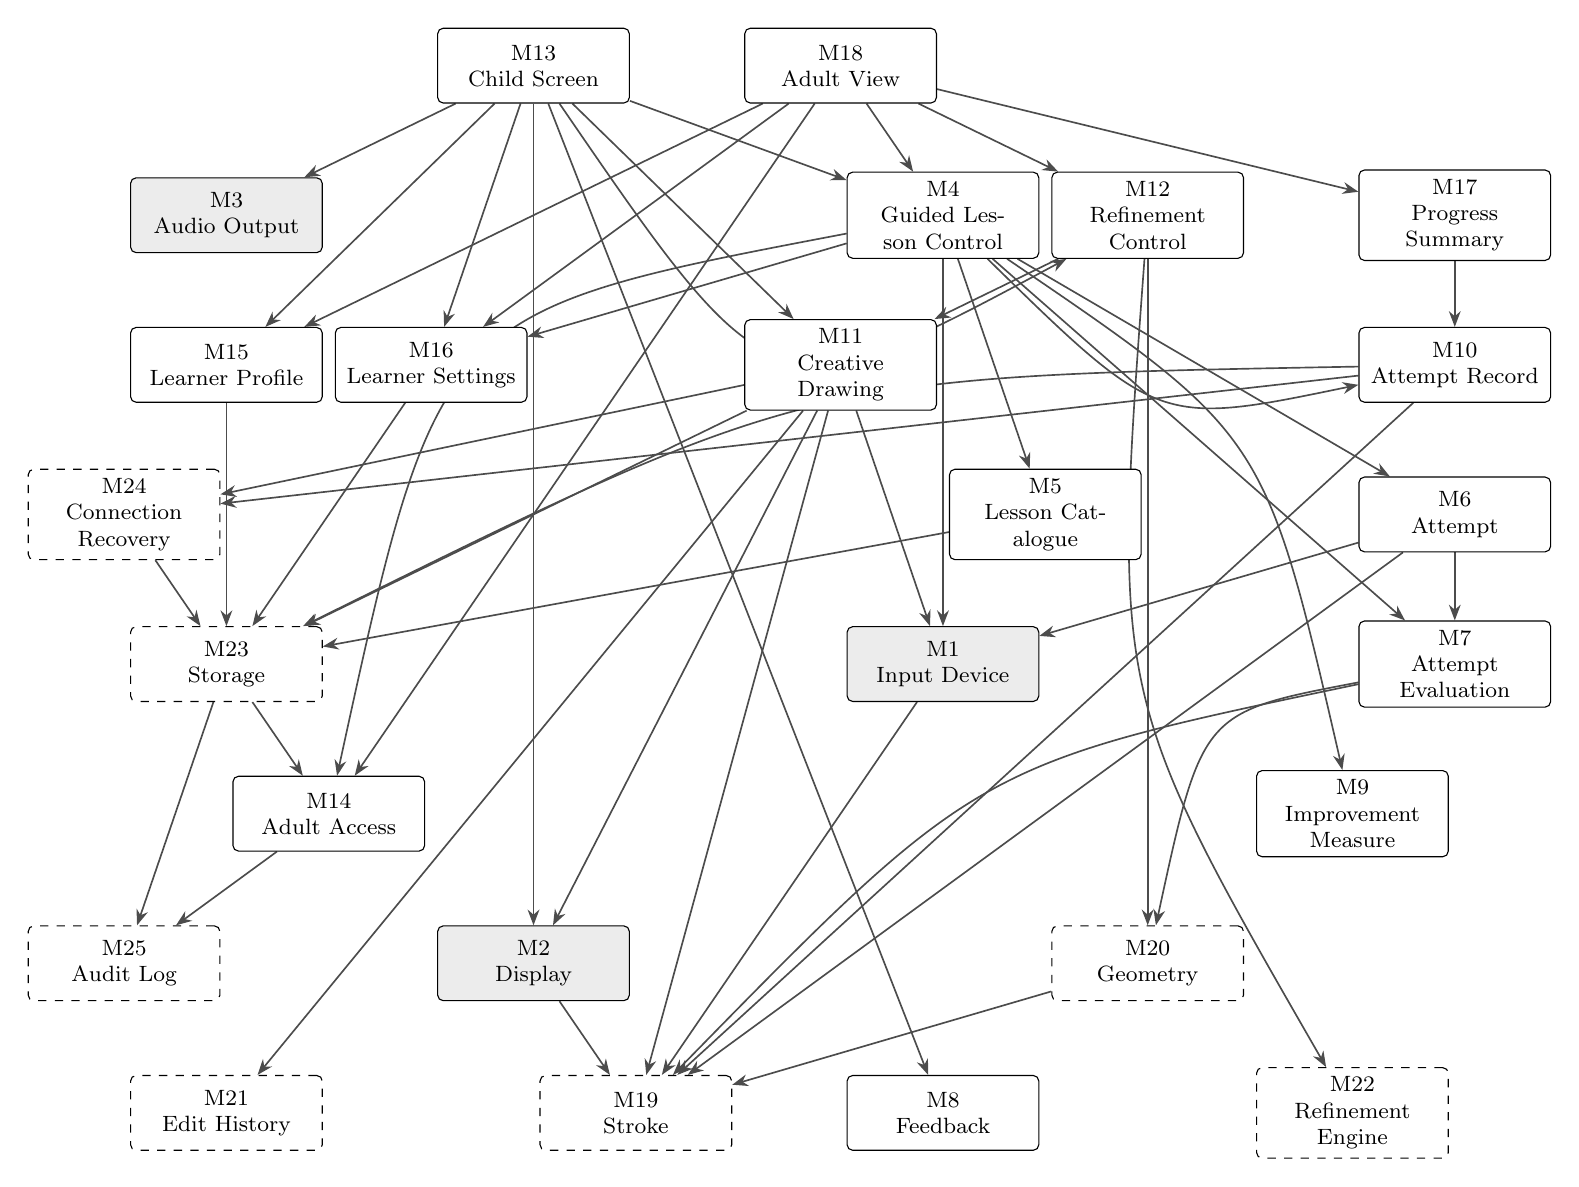
\begin{tikzpicture}[
  mod/.style={draw, rectangle, rounded corners=2pt, minimum width=2.3cm,
    text width=2.2cm, minimum height=0.95cm, align=center, font=\footnotesize,
    fill=white},
  hh/.style={mod, fill=gray!15},
  sd/.style={mod, dashed},
  use/.style={-{Stealth[length=2mm]}, semithick, draw=black!70}]
% Row 1
\node[mod] (m13) at (5.20,0.00) {M13\\Child Screen};
\node[mod] (m18) at (9.10,0.00) {M18\\Adult View};
% Row 2
\node[hh] (m3) at (1.30,-1.90) {M3\\Audio Output};
\node[mod] (m4) at (10.40,-1.90) {M4\\Guided Lesson Control};
\node[mod] (m12) at (13.00,-1.90) {M12\\Refinement Control};
\node[mod] (m17) at (16.90,-1.90) {M17\\Progress Summary};
% Row 3
\node[mod] (m15) at (1.30,-3.80) {M15\\Learner Profile};
\node[mod] (m16) at (3.90,-3.80) {M16\\Learner Settings};
\node[mod] (m11) at (9.10,-3.80) {M11\\Creative Drawing};
\node[mod] (m10) at (16.90,-3.80) {M10\\Attempt Record};
% Row 4
\node[sd] (m24) at (0.00,-5.70) {M24\\Connection Recovery};
\node[mod] (m5) at (11.70,-5.70) {M5\\Lesson Catalogue};
\node[mod] (m6) at (16.90,-5.70) {M6\\Attempt};
% Row 5
\node[sd] (m23) at (1.30,-7.60) {M23\\Storage};
\node[hh] (m1) at (10.40,-7.60) {M1\\Input Device};
\node[mod] (m7) at (16.90,-7.60) {M7\\Attempt Evaluation};
% Row 6
\node[mod] (m14) at (2.60,-9.50) {M14\\Adult Access};
\node[mod] (m9) at (15.60,-9.50) {M9\\Improvement Measure};
% Row 7
\node[sd] (m25) at (0.00,-11.40) {M25\\Audit Log};
\node[hh] (m2) at (5.20,-11.40) {M2\\Display};
\node[sd] (m20) at (13.00,-11.40) {M20\\Geometry};
% Row 8
\node[sd] (m21) at (1.30,-13.30) {M21\\Edit History};
\node[sd] (m19) at (6.50,-13.30) {M19\\Stroke};
\node[mod] (m8) at (10.40,-13.30) {M8\\Feedback};
\node[sd] (m22) at (15.60,-13.30) {M22\\Refinement Engine};
% Uses: an arrow from A to B means A uses B
\begin{pgfonlayer}{background}
\draw[use] (m13) -- (m4);
\draw[use] (m13) -- (m11);
\draw[use] (m13) .. controls (8.25,-4.45) .. (m12);
\draw[use] (m13) -- (m15);
\draw[use] (m13) -- (m16);
\draw[use] (m13) -- (m2);
\draw[use] (m13) -- (m3);
\draw[use] (m13) -- (m8);
\draw[use] (m18) -- (m4);
\draw[use] (m18) -- (m12);
\draw[use] (m18) -- (m14);
\draw[use] (m18) -- (m15);
\draw[use] (m18) -- (m16);
\draw[use] (m18) -- (m17);
\draw[use] (m4) -- (m1);
\draw[use] (m4) -- (m5);
\draw[use] (m4) -- (m6);
\draw[use] (m4) -- (m7);
\draw[use] (m4) .. controls (14.49,-4.68) .. (m9);
\draw[use] (m4) .. controls (13.14,-4.58) .. (m10);
\draw[use] (m4) .. controls (3.99,-3.12) .. (m14);
\draw[use] (m4) -- (m16);
\draw[use] (m12) -- (m11);
\draw[use] (m12) -- (m20);
\draw[use] (m12) .. controls (12.55,-8.00) .. (m22);
\draw[use] (m17) -- (m10);
\draw[use] (m11) -- (m1);
\draw[use] (m11) -- (m2);
\draw[use] (m11) -- (m19);
\draw[use] (m11) -- (m21);
\draw[use] (m11) -- (m23);
\draw[use] (m11) -- (m24);
\draw[use] (m10) -- (m19);
\draw[use] (m10) .. controls (8.67,-3.95) .. (m23);
\draw[use] (m10) -- (m24);
\draw[use] (m6) -- (m1);
\draw[use] (m6) -- (m7);
\draw[use] (m6) -- (m19);
\draw[use] (m5) -- (m23);
\draw[use] (m15) -- (m23);
\draw[use] (m16) -- (m23);
\draw[use] (m24) -- (m23);
\draw[use] (m7) .. controls (10.83,-8.87) .. (m19);
\draw[use] (m7) .. controls (13.69,-8.21) .. (m20);
\draw[use] (m23) -- (m14);
\draw[use] (m23) -- (m25);
\draw[use] (m14) -- (m25);
\draw[use] (m1) -- (m19);
\draw[use] (m2) -- (m19);
\draw[use] (m20) -- (m19);
\end{pgfonlayer}
\end{tikzpicture}}
\caption{Use hierarchy among modules. Shaded boxes are Hardware-Hiding modules,
plain boxes are Behaviour-Hiding modules and dashed boxes are Software Decision
modules. An arrow from A to B means A uses B.}
\label{FigUH}
\end{figure}

%\section*{References}

\section{User Interfaces}

\wss{Design of user interface for software and hardware.  Attach an appendix if
needed. Drawings, Sketches, Figma}

\section{Design of Communication Protocols}

\wss{If there is communication between hardware and software, it may be necessary 
to explain the design of the communication protocol.  This section should be filled 
in with NA if it is not appropriate for a given project.}

\section{Database Design}

\wss{If a database is a significant component of the project, the database
design should be summarized here.  This section should be filled in with NA if
it is not appropriate for a given project.}

\section{Timeline}

\wss{Schedule of tasks and who is responsible}

\wss{You can point to GitHub if this information is included there}

\section{Generative AI Use Disclosure}

\wss{ChatGPT (version 5) was used to brainstorm ideas for the template for this disclose section.}

\subsection{AI Tools Used}

\wss{Give the name of the AI tool(s) used and the version.}

\subsection{How and Where Used}

\wss{Explain what the tool(s) were used for.  Examples include: brainstorming,
explaining a technical concept, reviewing the document, generating or modifying
text, generating or modifying diagrams, identifying errors or omissions or
inconsistencies.}

\wss{For each of the uses, identify which parts of the document were affected.}

\wss{You do not need to report every interaction, but you should disclose the 
uses that materially contributed to your work}

\subsection{Verification of AI-Generated Content}

\wss{\begin{itemize}
    \item Describe how the team checked AI-generated or AI-assisted material
    before including it in the document.
    \item In particular, verify factual claims, technical assertions,
    requirements, calculations, references, and other information for which an
    AI system may produce incorrect or fabricated results.
    \item \textbf{The team is responsible for the accuracy, completeness,
consistency, and appropriateness of the submitted document, regardless of
whether material was generated by a human or an AI system.}
\end{itemize}}

\newpage{}

\bibliographystyle {plainnat}
\bibliography{../../../refs/References}

\end{document}